\documentclass[11pt]{article}

\usepackage[margin=1in]{geometry}
\usepackage[colorlinks=true]{hyperref}
\usepackage{graphicx}
\usepackage{listings}
\usepackage{siunitx}
\usepackage{sidecap}
\usepackage{float}


\lstset{language=R}



\begin{document}


ME 331 11am ThermoFluids

Marcus Hall 

Experimental Wind Tunnel Project

\today

\medskip\hrule\medskip

\begin{enumerate}
\item The top two plots are the Rough and Smooth data from a group in the 8 am, were the bottom two are the Rough and Smooth plots from the first group in the 11 am class. The differencation between the left and right are the right two plots are with all the units converted to English and then reduced down, were the left two are converted to Metric and then reduced down. Even though coeffeint of drag is unit less along with Reynolds number, the units that the calcuations were done in gave different ranges, but had consitant shape. The reason for this is unknown. Both the English and Metric was off a couple of magnitudes from the ``true'' value of about $10^5$. The Metric was lower than the ``true'' and the English was higher then the ``true''.\\
The reason 2 differnet data sets were used, was due to the 11 am data not having a distinousable drop to see were the laminar flow turned in to turbulent.   
\begin{figure}[h]
\centering
  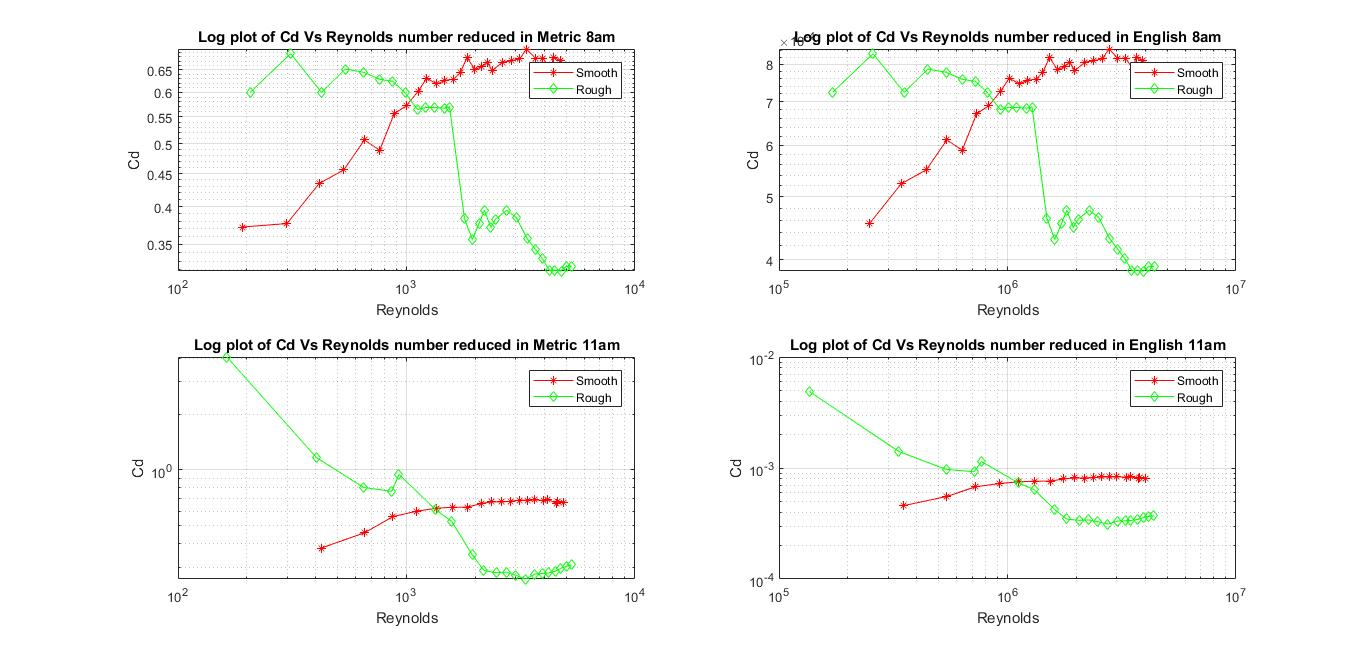
\includegraphics[width =7in]{x4.jpg}
  \caption{Coeffient of Drag versus Reynolds number}
  \label{fig:Cd}
\end{figure}

\item $Re_{critical} = 1.5e6 $ \\
	$\frac{\epsilon}{D} = $


\item 

\item The Reynolds number is a determination at were the flow transistions from
laminar to turbulent flow. The main reason that a flow becomes turbulent is that the
fluid is moving to fast for it to move smoothly around an object . Momentum of fluid
around a radius The $C_d$ becomes lower because the separation point moves further
back on the sphere, causing the flow to move in a smoother path. Size of the wake.
Differnce in pressures \\
At low Reynolds number, the cylinder acts as a blunt body, resulting in a higher
$C_d$ 


\begin{figure}[h]
\centering
  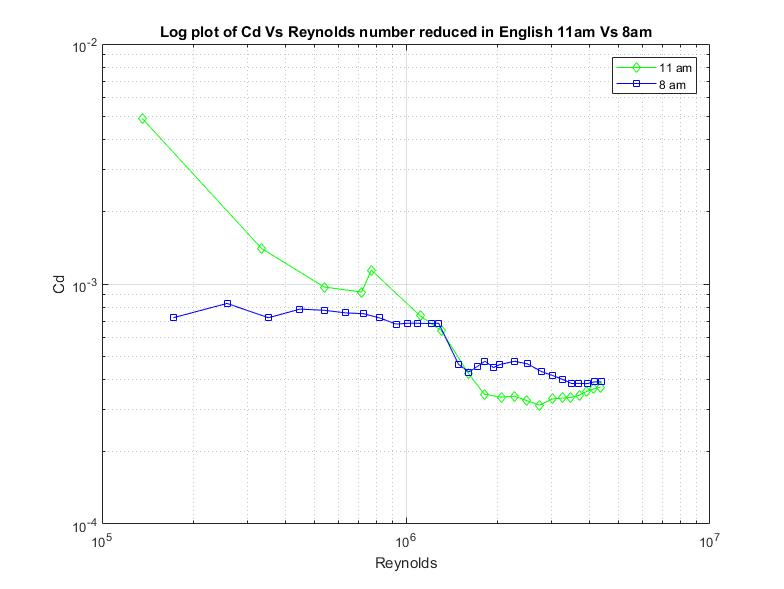
\includegraphics[width =7in]{combined.jpg}
  \caption{Coeffient of Drag versus Reynolds number of 2 different data sets}
  \label{fig:Cdx2}
\end{figure}

\end{enumerate}

\end{document}